\documentclass[10pt,twocolumn]{IEEEtran}
% replace the keyword "twocolumn" by "onecolumn" if you want a single column document

% ------------------------------------------------------------------------------------
% If you are using *TeXnicCenter*, already configured with profiles as "LaTeX -> PDF",
% do the following to create a project and have the compile hotkey Ctrl+F5:
%     Project -> Create with active file as the main file
% Do not forget to select "Uses BibTeX"
% ------------------------------------------------------------------------------------

% some useful packages:
\usepackage{graphicx}
\graphicspath{{./}{./figs/}{../figs/}{../figs/w13/}} % share figs using ../figs/
\usepackage{url}
\usepackage{amsmath}

\begin{document}

\title{Report on dataset generation and methodology}
\author{Jose Pedro Gomes}

\maketitle

\begin{abstract}
    Documentation on how the data was acquired and of the experimental setup used.
\end{abstract}

\section{Introduction}

In order to test the proposed and implemented solutions, data is necessary. Due to its novelty, event cameras have very few datasets available publicly, and none of which suited for our case study of the eye saccades. As such, for this work, it was necessary to generate the data being used. Both synthetic and real world datasets were produced. The relevant sensor data that was captured was image frame, event, and IMU sensor information (as well as camera calibration information). Furthermore, in order to validate the results obtained, the real (groundtruth) information pertaining to pose was also recorded, to later be compared with the estimated results obtained. 


\section{Method}

This section aims to explain the different methods used to acquire and generate datasets, namely synthetic data (\ref{sec:w13_synthetic}), real data from other research groups that is publicly available (\ref{sec:w13_datasets}) and the real data that we generated for this work and have mad epublicly available (\ref{sec:w13_kinova}). 

\subsection{Synthetic data}
\label{sec:w13_synthetic}

ESim (ref here) was used to generate a simulated, synthetic dataset. This dataset simulates a DAVIS240 camera with both frames and events simultaneously, as well as IMU and camera calibration information. Furthermore, groundtruth values are also provided, containing the pose (position and orientation) of the simulated camera at each instant. This scenario consists of a living room rendered using Unreal Engine for increased visual realism, with sensor information being generated by ESim. A plethora of trajectories was generated, starting from single axis, no noise movement, all the way to multi axis translation and rotation, with camera noise, motion blur, and IMU biases. 

Though the transference from simulated to real scenarios is not exact, the synthetic datasets nevertheless provide a controlled scenario that is useful to test multiple algorithms, not only limited to the case study of this work, such as image reconstruction and egomotion estimation from events, to name two.

A sample scene from the dataset is shown in Fig\,\ref{fig:w13_synthetic}. For a more in-depth explanation on how to generate trajectories, refer to (insert appendix refernce here).

\begin{figure}[ht]
    \centering
    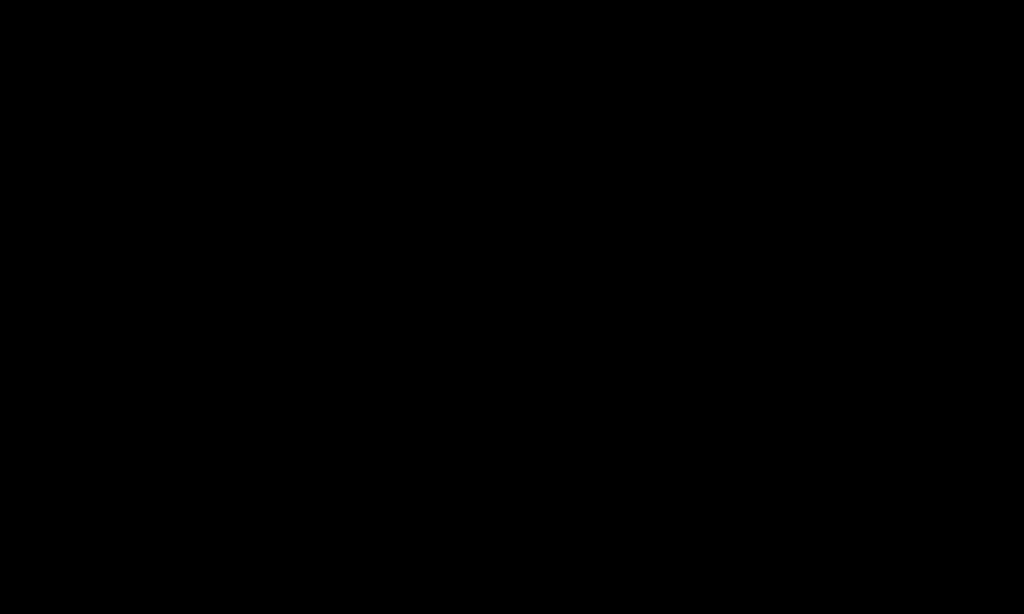
\includegraphics[width = 1\linewidth]{placeholder.png}
    \caption[]{placeholder}
    \label{fig:w13_synthetic}
\end{figure}

Furthermore, we can generate high speed movement compatible with saccadic eye movement, as desired by our work.

\subsection{Community datasets}
\label{sec:w13_datasets}

The Depts. Informatics and Neuroinformatics at ETH Zurich provides a set of event camera datasets, recorded with a DAVIS 240C (an event camera with both events and full frames), along with IMU measurements and ground truth  (position and orientation) from a motion-capture system. 

These datasets contain various scenarios and trajectories, with multiple complexities, from poorly textured environments to more complex ones, with simple trajectories (rotation-only or translation-only) to compound movement. However, the movement generation is not precise, as they were captured by randomly moving the camera by hand (as such neither are the translation-only trajectories free from a small rotation nor vice-versa). 

Therefore, these datasets, though accompanied by high quality ground truth obtained through motion capture, were not exactly suited for our work. Nevertheless, these datasets were udeful to test our implemenation on other scenarios, as well as compare performance with other implementations that provided results using the same datasets.

The sensor information contained is similar to the synthetic dataset. Fig\,\ref{fig:w13_shapes} shows a sample frame from one of these datasets, showcasing a carefully controlled and textured environment.

\begin{figure}[ht]
    \centering
    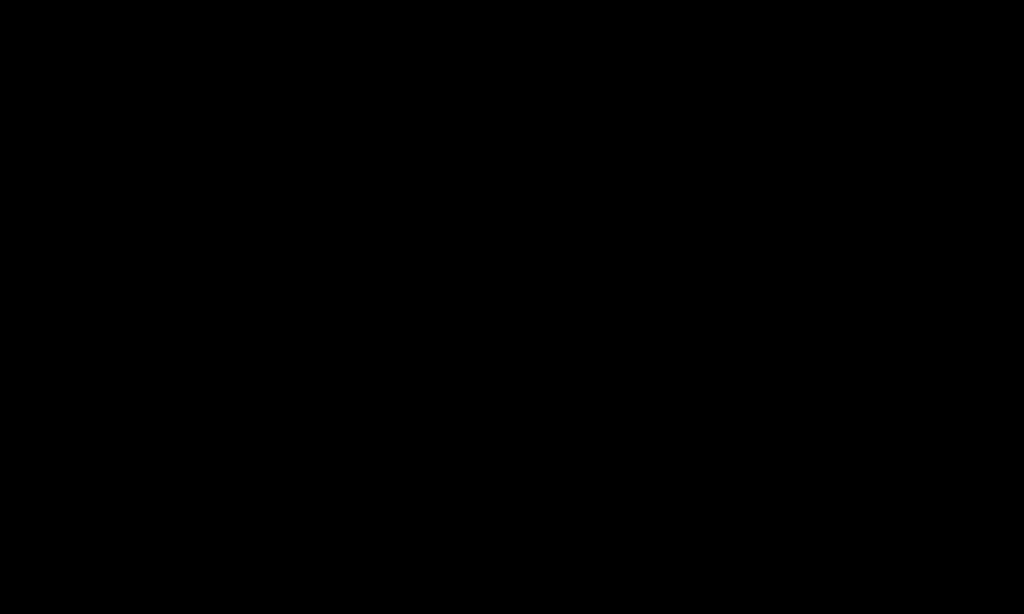
\includegraphics[width = 1\linewidth]{placeholder.png}
    \caption[]{placeholder}
    \label{fig:w13_shapes}
\end{figure}

\subsection{Datasets produced (Kinova and Optitrack)}
\label{sec:w13_kinova}

Since the datasets using real sensors were not perfectly suited for ou case study, we recorded our own. The sensor used consisted of the following: 1) a DVS240 camera, 2) Optitrack motion capture system, and 3) Kinova robotic arm.

The DVS240 event camera was used for visual and inertial information. Since this camera does not allow for simultaneous recording of both events and frames, two situations were created: 1) switching to frame-mode when the camera is stopped, and to events-mode when it is moving, and 2) start recording in frame-mode, and switch to event-mode when the camera starts moving (and keep it in this mode until the end of the recording). These two modes were chosen in accordance with implementation suggestions for our case study. Inertial measurements were generated thorugh the embedded IMU senor in the camera, aligned with the optical centre.

The Kinova robotic arm objective is twofold: 1) provide a way to generate a very controlled trajectory, which was carefuly created to replicate a saccadic eye movement, and 2) provide information on the ground truth pertaining to pose. For information on the Kinova arm, as well as trajectory generation, refer to the Appendix (insert reference here). 

The Optitrack motion capture system was used as a way to have independent and redundant ground truth information on the state of the camera.

Fig\,\ref{fig:w13_kinova_setup} shows the setup used, with the Kinova arm gripping the DVS240 event camera on its end.

\begin{figure}[ht]
    \centering
    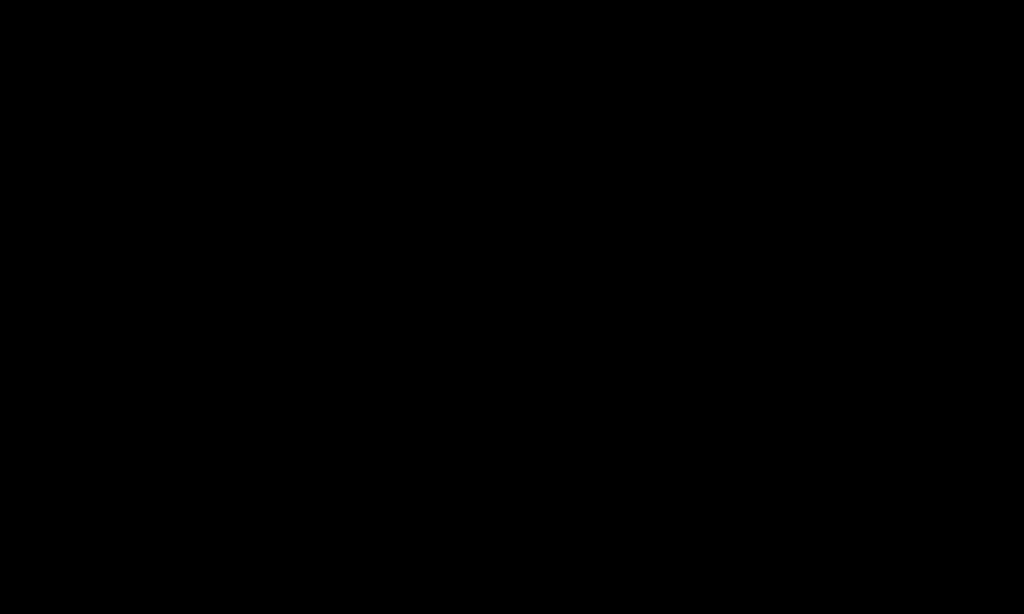
\includegraphics[width = 1\linewidth]{placeholder.png}
    \caption[]{placeholder}
    \label{fig:w13_kinova_setup}
\end{figure}

However, this setup is not perfectly representable of our case study, in particular due to physical limitation of the robot arm, as the maximum velocities and accelerations that can be generated do not come close to those generated during a normal saccadic eye movement. Nevertheless, this approach was the closest achievable given the available hardware.


%\bibliographystyle{plain}
%\bibliography{../thesis/ref}
% replace "project" by "thesis" if you are doing the thesis

\end{document}
